\documentclass[a4paper]{article}
\usepackage[normalem]{ulem}
\usepackage[english]{babel}
\usepackage[utf8x]{inputenc}
\usepackage{amsmath}
\usepackage{graphicx}
\usepackage[colorinlistoftodos]{todonotes}

\usepackage{amssymb,amsmath,amsthm,amsfonts}
\usepackage{calc}
\usepackage{graphicx}
\usepackage{subfigure}
\usepackage{gensymb}
\usepackage{natbib}
\usepackage{url}
\usepackage[utf8x]{inputenc}
\usepackage{amsmath}
\usepackage{graphicx}
\graphicspath{{images/}}
\usepackage{parskip}
\usepackage{fancyhdr}
\usepackage{vmargin}
\usepackage{algorithm}
\usepackage{enumitem}
\linespread{1}
\usepackage{color}
\usepackage{cite}
\usepackage{amsmath,amssymb}
\newtheorem{claim1}{Claim}
\usepackage{algpseudocode}% http://ctan.org/pkg/algorithmicx
\usepackage[compatibility=false]{caption}% http://ctan.org/pkg/caption
\setmarginsrb{3 cm}{2.5 cm}{3 cm}{2.5 cm}{1 cm}{1.5 cm}{1 cm}{1.5 cm}

\title{Lecture Notes}					% Titulo
\author{Malgudi Labs}					% Autor
%\date{\today}						% Fecha


\makeatletter
\let\thetitle\@title
\let\theauthor\@author
%\let\thedate\@date
\makeatother

\pagestyle{fancy}
\fancyhf{}
\rhead{\theauthor}
\lhead{\thetitle}
\cfoot{\thepage}

\begin{document}

%%%%%%%%%%%%%%%%%%%%%%%%%%%%%%%%%%%%%%%%%%%%%%%%%%%%%%%%%%%%%%%%%%%%%%%%%%%%%%%%%%%%%%%%%

\begin{titlepage}
	\centering
    \vspace*{0.0 cm}
    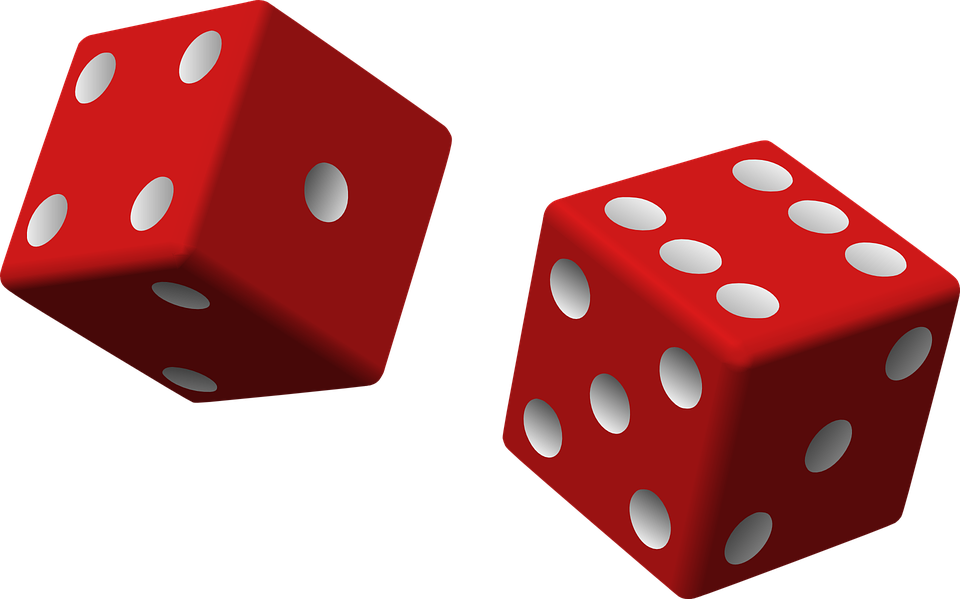
\includegraphics[scale = 0.1]{dice.png}\\[.0 cm]	% Logo Universidad
    \textsc{\LARGE Probability and Computing}\\[2.0 cm]	% Nombre Universidad
	\textsc{\Large CSL-471}\\[0.5 cm]				% Codigo Curso
	\textsc{\large Instructor: Dr. Sudarshan Iyengar}\\[0.5 cm]		% Nombre Curso
	\rule{\linewidth}{0.2 mm} \\[0.4 cm]
	{ \huge \bfseries \thetitle}\\
	\rule{\linewidth}{0.2 mm} \\[1.5 cm]
	
	\begin{minipage}{0.4\textwidth}
		\begin{center} \large
			\emph{Author:}\\
			\theauthor\linebreak
			\end{center}
	\end{minipage}\\[2 cm]
	
%	{\large \today}\\[2 cm]
 
	\vfill
	
\end{titlepage}

%%%%%%%%%%%%%%%%%%%%%%%%%%%%%%%%%%%%%%%%%%%%%%%%%%%%%%%%%%%%%%%%%%%%%%%%%%%%%%%%%%%%%%%%%

\tableofcontents
\pagebreak

%%%%%%%%%%%%%%%%%%%%%%%%%%%%%%%%%%%%%%%%%%%%%%%%%%%%%%%%%%%%%%%%%%%%%%%%%%%%%%%%%%%%%%%%%

\section{ Puzzle 1. The Monty Hall Problem:}

The Monty Hall problem is based on the American reality show - ``Let's make a deal'' and is named after its host, Monty Hall. 

Consider a scenario where there are 3 doors. One door contains BMW car and other 2 contain goats. Your goal is to choose one door and if the door has BMW hidden inside, you win. 

In this case, probability of winning a BMW = 1/3, probability of losing=2/3.\\

\textbf{But, the Monty Hall Game introduces a twist here.}\\

Suppose Monty Hall enters the scene. He asks you to choose one door. You choose. After asking the choice of your door, out of the remaining two doors, he opens the one which has goat\footnote{Monty knows which door has what. That's why he is capable of opening a door which has a goat hidden.}. After showing you, out of the remaining two doors, which has the goat, he asks you if you want to change your choice and choose the third gate which is unopened and previously not chosen by you. This has been shown in Figure \ref{monty} \\

\begin{figure}[h]
\centering
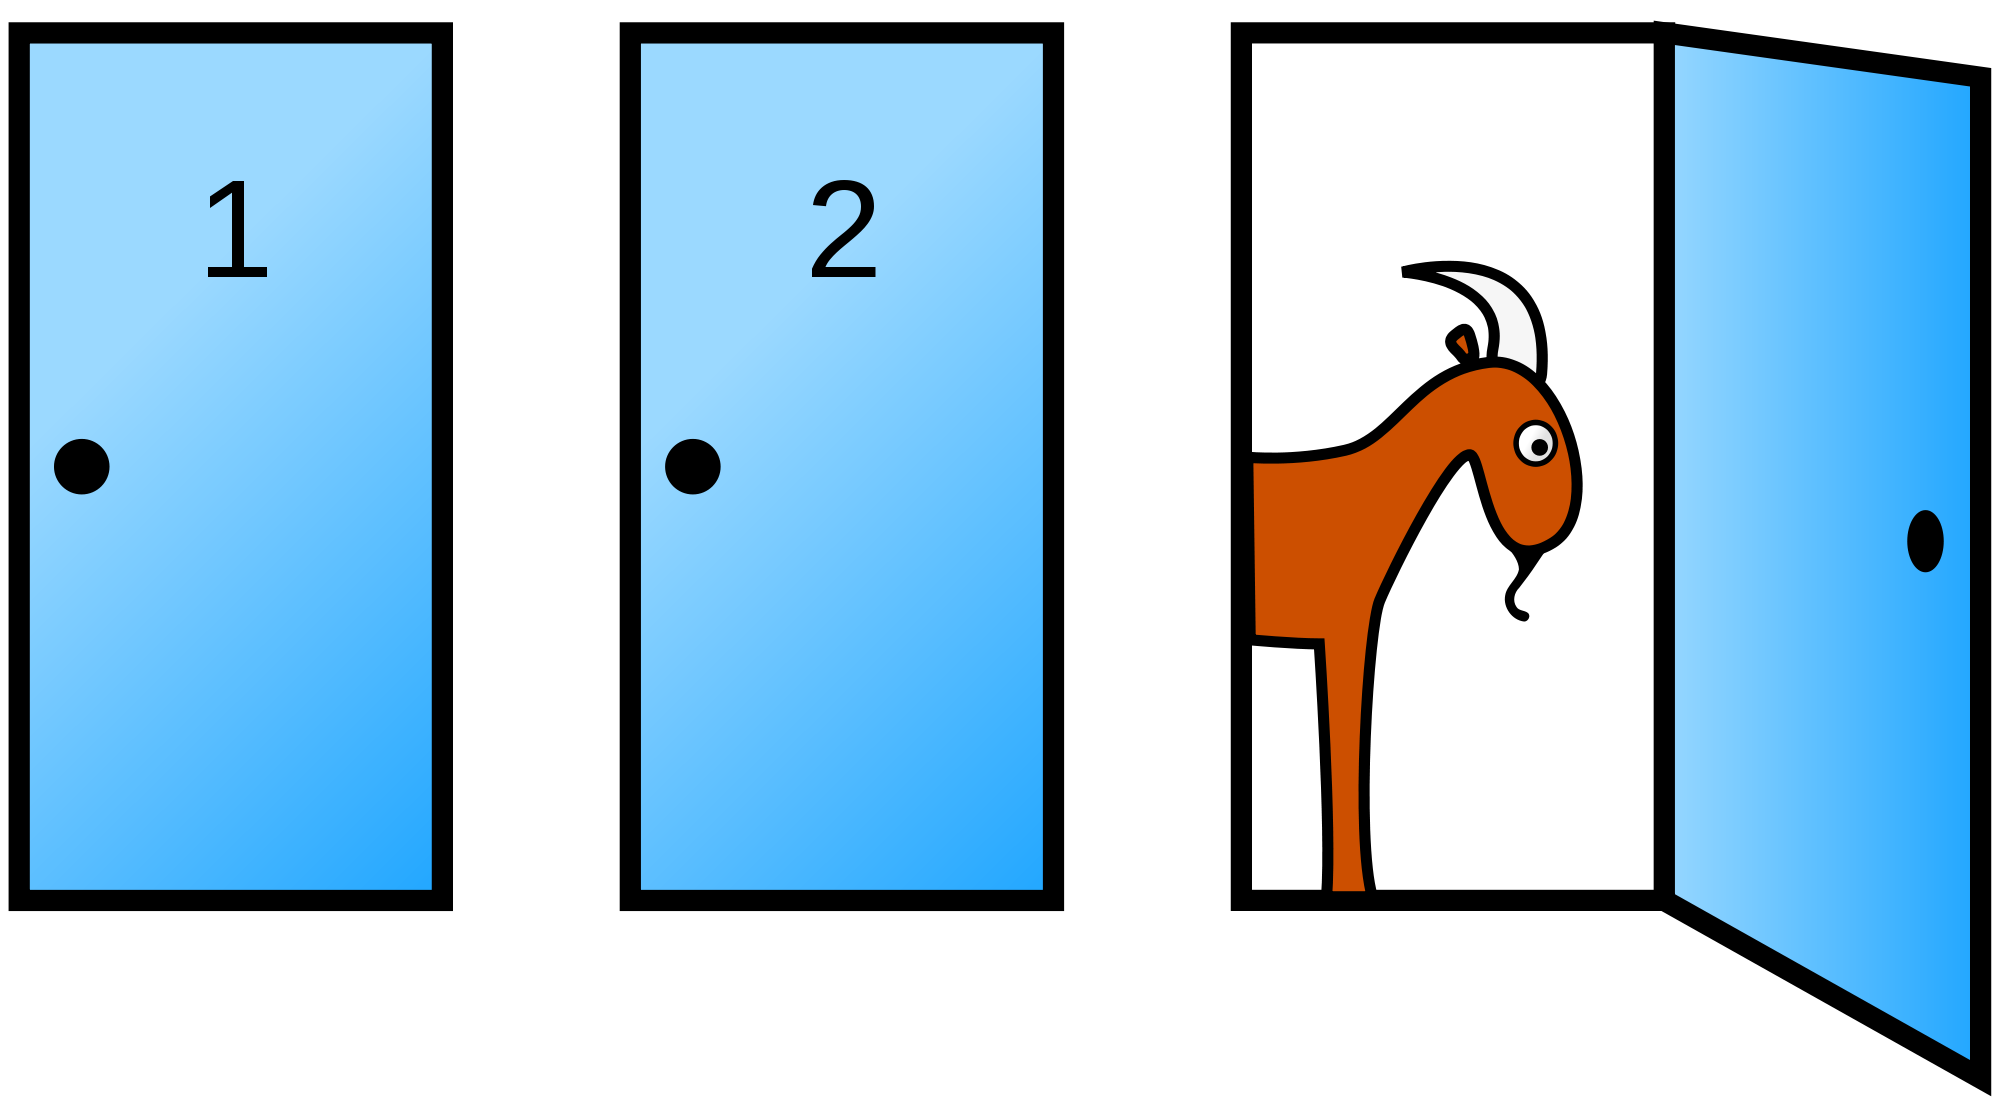
\includegraphics[width=0.5\textwidth]{monty.png}
\label{monty}
\caption{The Monty Hall Game}
\end{figure}

\textit{SHOULD YOU SWAP? Does swapping make any difference to your probability of winning? }

Case 1: You do not swap: So, you have chosen one door and after knowing which of the other two doors has a goat, you do not swap your choice. So, this extra knowledge does not matter to your answer.
Hence, Probability (Win) = 1/3 and Probability (Losing) = 2/3

Case 2: You swap: 
Case 2.a : You have chosen the door hiding a goat previously: 
Probability (You have chosen the door hiding goat) = 2/3. Now Monty shows you the other door having a goat. So, when you swap, you definitely pick the door having BMW. Hence, your probability of winning = 2/3.

Case 2.b : You have chosen the door hiding BMW previously: 
Probability (You have chosen the door hiding BMW) = 1/3. Now Monty shows you the other door having a goat. So, when you swap, you definitely pick the door having another goat. Hence, your probability of losing= 1/3.

Thus, you should always swap.

\textbf{Quick Brainteaser}:What is the probability of winning if participant tosses an unbiased coin. If head comes, she swaps, else does not swap? \\
Answer:1/2 \\


\section{Puzzle 2: The Coin Tossing Show}
\textbf{The Game}: In a contest, a participant tosses a coin until he gets first head. He wins cash amount of $100 \times number\ of\ coins\ tossed$. What is the expected value of cash price won by the participant?\\

\textbf{Answer}: 
Let $X$ be a random variable which counts the number of tosses to get the first head.\\

We know that $X$ can take the values 1, 2, 3, 4.......\\
$E[X]\ =\ 1 \times pr(X=1) + 2 \times pr(X=2) + 3 \times pr(X=3)+ .... $\\

= $\sum_{i=1}^{\infty} i \times pr(X=i) $\\

Since, $ pr(X=i) $ = $(1/2)^i$\\

Hence, $E[X]\ = \sum_{i=1}^{\infty} i/2^{n} $\\

= $1/2+(2/2^2)+(3/2^3)+(4/2^4)+.....\ =\ \alpha$, say\\

Now, $\alpha = 1/2+(2/2^2)+(3/2^3)+(4/2^4)+.....$(1)\\

$\alpha/2 = (2/2^2)+(3/2^3)+(4/2^4)+.....$(2)\\

Subtract 2 from 1 \\

$\alpha/2= (1/2)+(1/2^2)+(1/2^3)+.....$\\

It can be seen that it is a geometric progression $a,ar,ar^2,ar^3......$, with $a=1$ and $r=1/2$.\\

We know, that the sum of an infinite Geometric Progression = $\frac{a}{1-r}$ = $\frac{1/2}{1-1/2}$ (in this case) = $1$. \\

Hence, $\alpha/2\ = 1$\\

$\alpha=2$\\

$E[X]=2$\\  	(3)

So, the expected amount of money won by the participant = $2 \times 100$ \$ = $200$ \$.\\

Now, we know that the expected amount of money won by the participant is $200$ \$. But, when the game is actually played, the participant can win $100$ \$ in one case, yet $500$ \$ in other case, yet $10000$ \$ in other case. Hence, it is important to look at the standard deviation of the random variable $X$, in addition to its expected value.\\

The formula for Standard Deviation, $\sigma(X)$, is given as :\\ 

$\sigma(X)$= $ \sqrt{(E[X- \mu])^2} $, where $\mu = E[X]$\\


= $ \sqrt{E[X^2 - 2 X \mu + \mu ^ 2]} $\\

= $ \sqrt{E[X^2 ]- 2 E[X] \mu + E[\mu ^ 2]} $\\

= $ \sqrt{E[X^2 ]- 2 \mu^2 + \mu ^ 2} $\\

= $ \sqrt{E[X^2 ]- \mu ^ 2} $\\

= $ \sqrt{E[X^2 ]- (E[X]) ^ 2} $\\

Hence, $\sigma(X)$=  $ \sqrt{E[X^2 ]- (E[X]) ^ 2} $	(4)\\

$X^2$ is also a random variable, which takes the values $1^2, 2^2, 3^2, 4^2..........$\\

$Pr(X^2=1^2) = Pr(X=1) = 1/2$\\

$Pr(X^2=2^2) = Pr(X=2) = 1/2^2$\\

... and so on \\

According the the expectation formula, $E[X^2] = 1^2 \times \frac{1}{2} + 2^2 \times \frac{1}{2^2} + 3^2 \times \frac{1}{2^3} + ............  $ = $\alpha$ say\\

$\alpha\ =\ \frac{1^2}{2^1} + \frac{2^2}{2^2} + \frac{3^2}{2^3} + \frac{4^2}{2^4} + .... $   (5) \\	


$\alpha/2\ =\ \frac{1^2}{2^2} + \frac{2^2}{2^3} + \frac{3^2}{2^4} + \frac{4^2}{2^5} + .... $   (6)  \\

Subtract (6) from (5)\\

$\alpha/2\ =\ \frac{1^2}{2^1} + \frac{2^2-1^2}{2^2} + \frac{3^2-2^2}{2^3} + \frac{4^2-3^2}{2^4} + .... $    \\


or, $\alpha/2\ =\ \frac{1^2}{2^1} + \frac{(2+1)(2-1)}{2^2} + \frac{(3+2)(3-2)}{2^3} + \frac{(4+3)(4-3)}{2^4} + .... $    \\


or, $\alpha/2\ =\ \frac{1}{2^1} + \frac{3}{2^2} + \frac{5}{2^3} + \frac{7}{2^4} + .... $     (7)\\	

Divide by 2\\

 or, $\alpha/4\ =\ \frac{1}{2^2} + \frac{3}{2^3} + \frac{5}{2^4} + \frac{7}{2^5} + .... $  (8)\\
 
 Subtract (8) from (7)\\
 
$\alpha/4\ =\ \frac{1}{2} + \frac{2}{2^2} + \frac{2}{2^3} + \frac{2}{2^4} + .... $\\

or, $\alpha/4\ =\ 1 + \frac{1}{2^2} + \frac{1}{2^3} + \frac{1}{2^4} + .. $\\ 

or, $\alpha/4\ =\frac{3}{4}$, (applying the formula for sum of Geometric Progression)\\

$\alpha = 6$, \\

$E[X^2]=6$	(9)\\

Putting 3 and 9 in 4, $\sigma(X)$=  $ \sqrt{6- 2 ^ 2} $\\

= $\sqrt{2}$\\	
\textbf{Brain Teaser}: 1. State whether series is convergent $\sum_{n=1}^{\infty} n/2^{n} $\\
2. State whether the series is convergent $\sum_{n=1}^{\infty} 1/n$ \\


\section{Some interesting math jokes and to be thought about questions}

{\footnotesize These paradoxes have not been discussed in detail in the class. They will be covered in the tutorial session.}

\begin{enumerate}

\item A mathematician was caught hiding a bomb in his bag while boarding onto the flight from England to Canada. When asked why he has done so, he says - ``The probability of a man carrying a bomb in a flight = $\frac{1}{1000}$, which is still very high. So I could not have my peace of mind on the journey. But the probability of two people carrying a bomb in the flight = $\frac{1}{1000} \times \frac{1}{1000}\ = \frac{1}{1000000}$, which is very less. So if I carry a bomb, the probability of another bomb being present in this flight reduces by a very big extent."\\
\textit{To think:}What is wrong about these reasoning. 

\item Imagine a very old building standing intact from millions of years. Let $P(today)$ = The probability that this building will fall today and $P(tomorrow)$ = The probability that this building will fall tomorrow. \\
\textit{To think}: Whether $P(today)<P(tomorrow)$, or $P(today)>P(tomorrow)$ or $P(today)=P(tomorrow)$ ?

\item Consider a multiple choice exam conducted countrywide. There are two students- $A$ and $B$. $A$ and $B$ both have got equal marks. But $A$ knew the answers correctly of the questions he answered, while $B$ answered the questions randomly and was lucky enough to get the same marks as $A$. \\
\textit{To think:} By looking at their OMR\footnote{Optical Mark Reading- One where we darken the bubbles corresponding to the correct answer- A/B/C/D.} sheets, can you tell, which is the sheet of $A$ and which is the sheet of $B$.

\end{enumerate}


\section{Online Hiring/ Dating Problem}
\textbf{Problem Statement}: You are searching for a match for marriage. There are $1000$ boys standing in a row, and you have to choose one out of them. According to the rules of the game, you can interview the boys only in a sequence one by one. If the sequence is : \\ $B_1\ B_2\ B_3\ B_4\ B_5\ ....... \ B_{1000}\ $, you will first see $B_i$, only then $B_{i+1}$. You have a choice to accept or reject a boy. If you accept one, the game gets over and you tie a knot with the selected individual. If you reject a boy, you can not return back to him. He is gone forever. What should be the optimal strategy to choose as best person as possible?  

\textbf{Solution:} \\
\textit{Intuition:} Check out on some people. This will give you an idea of what the crowd is like. After getting the idea of the crowd, it will be easier to choose the best person. \\

Look for the first $k$ boys. Let $B_k$ be the best among these. Reject all of these $k$ boys and keep a note of $B_k$. After k boys, as soon as you see a boy better than $B_k$, you accept. This has been shown in Figure \ref{boy}.

\begin{figure}[h]
\centering
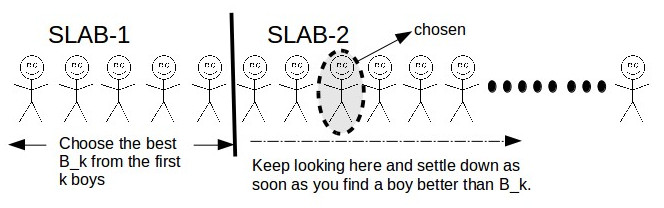
\includegraphics[width=0.9\textwidth]{boys.jpg}
\label{boy}
\caption{The technique to choose as best boy as possible}
\end{figure}

As an intelligent reader can make out, the value of $k$ plays a significant role here. If the value of $k$ is very small, you will end up choosing an inferior quality boy, since you have not seen enough samples. If $k$ is very big, not enough boys will be left in slab 2 to take a proper decision. So, now we look at the question - What should be the value of $k$.\\

Let $f(k)$ denote the quality of the selected boy when the first $k$ boys are employed as the sample of the entire population of available choices. We can plot a curve with $k$ on the X axis and $f(k)$ on the Y axis\footnote{Try writing a piece of code and observe how this plot looks like}. The roots of the equation $f'(k\ =0)$ give us the value of $k$ for which $f(k)$ is maximum, or in other words, we get the highest quality boy. This has been explained in detail in Algorithm \ref{dating}.

\begin{algorithm}
\caption{The Dating Algorithm}\label{dating}
\begin{algorithmic}[1]
\Procedure{Dating}{}
\State \textbf{Input}:- Array of the quality of $n$ boys $A[1,2,.....,n]$, $A[i]$ represents the quality of the $i_{th}$ boy, $k$
\State \textbf{Output}: $A[Best]$- The quality of the solution, $Best$- The index of the selected boy.
\State $Best\ = 0$
\For {$i\ =\ 1\ to\ k$}
\If {$A[Best] < A[i]$}
\State $Best \gets i $
\EndIf
\EndFor
\For {$i = k+1\ to\ n$}
\If {$A[Best] < A[i]$}
\State $Best \gets i$
\State break
\EndIf
\EndFor
\State return $Best$, $A[Best]$
\EndProcedure
\end{algorithmic}
\end{algorithm}

\subsection{Probability that Algorithm \ref{dating} fetches you the best boy}

The algorithm fails to fetch the best boy when one of the following two events occur.
\begin{itemize}
\item When the best boy is in the first $k$ boys(Our sample of the crowd). It is because, according to the algorithm the first $k$ boys are rejected and hence the best boy will also be rejected.  
\item When we pick a boy after the first $k$ boys and he is non-best. This is shown in Figure \ref{hero}. Here, we end up picking a suboptimal boy which is sandwiched between the $k+1_{th}$ location boy and the best boy. 
\end{itemize}

\begin{figure}[h]
\centering
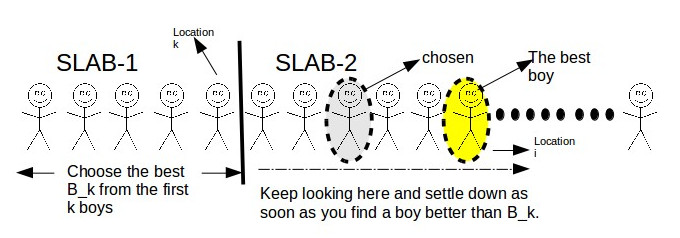
\includegraphics[width=0.9\textwidth]{hero.jpg}
\label{hero}
\caption{Choosing someone who is not the best}
\end{figure}

$Pr$(Best boy is in the first $k$ locations) = $ \frac{k}{n}$, since there are $k$ ways in which the best boy can be present at any of the first $k$ locations and the total number of locations to be present at are $n$. \\

We call a boy to be the pseudo-best if its quality is greater than $B_k$ and lesser than the quality of the best boy.
 
For the algorithm to fetch the best boy
\begin{enumerate}
\item The best boy should be present after the first $k$ locations. 
\item If the location of the best boy is $i$, no pseudo-best boy should be picked from the locations $[k+1,i-1]$.
\end{enumerate}


Hence, $Pr$(We get the best boy)= $Pr$(Best boy is at the location $i$ and no pseudo-best boy is present in the location $[k+1,i-1]$ ).\\

Given a location $i$, $Pr$(Best boy is present at this location) = $1/n$. \hspace{2mm} ....(1)\\

$Pr$(Pseudo-best boy is not there at locations $[k+1,i-1]$) = $\frac{k}{i-1}$. \hspace{2mm} ...(2) 

Why? Let us see.\\ 
We now, divide the queue of boys in three slabs as shown in Figure \ref{slabs}.

\begin{figure}[h]
\centering
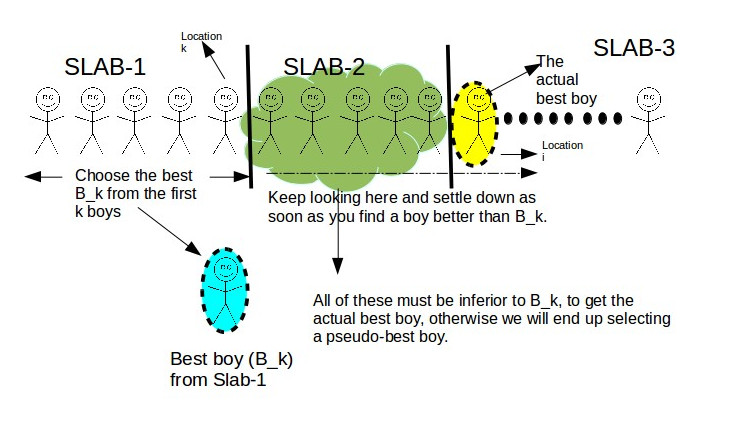
\includegraphics[width=0.9\textwidth]{slabs.jpg}
\label{slabs}
\caption{Choosing the best}
\end{figure}

$Pr$(The best boy from locations $1$ to $i-1$ is present before the location $k+1$)= $\frac{k}{i-1}$

From (1) and (2), \\
$pr$(winning when the best boy is at the location $i$) = $\frac{1}{n} \times \frac{k}{i-1}$\\

Now the location of the best boy can vary from $k+1$ to $n$. We have to take all these cases in account. \\

$Pr$(We end up choosing the best boy)= $\sum_{i=k+1}^n \frac{1}{n} \times \frac{k}{i-1}$\\

= $\frac{k}{n} \sum_{i=k+1}^n \frac{1}{i-1}$\\

= $\frac{k}{n} \sum_{i=k}^{n-1} \frac{1}{i}$\\

= $\frac{k}{n} \int_{k}^{n} \frac{1}{i} di$ (we replaced $n-1$ by $n$ assuming $n$ is a very large number)\\

= $\frac{k}{n}|log\ i|_{k}^{n}$\\

=$\frac{k}{n} (log\ n - log\ k)$\\

\[
 \boxed{f(k)\ =\ \frac{k}{n} (log\ n - log\ k)}
 \]
 
 Differentiating \\
 
 $f'(k)=\ \frac{1}{n} (log\ n\ -\ log\ k) + \frac{k}{n} \times \frac{-1}{k}$\\
 
 Equate to $0$. \\
 
 $\frac{1}{n} (log\ n\ -\ log\ k) + \frac{k}{n} \times \frac{-1}{k}\ =0$\\
 
 $ (log\ n\ -\ log\ k\ -\ 1\ = 0)$\\
 
 or, $log\ n\ -\ log_e\ e\ =\ log\ k$\\
 
 or, $log\ \frac{n}{e}\ =\ log\ k$\\
 
 or, 
\[
 \boxed{k=\ \frac{n}{e}}
 \]


\section{Lecture 3}

The main aim of this lecture is to understand the cryptanalysis of the Vigenere cipher. But before that, we will get a hint of the previous basic cryptographic techniques as well. 

\subsection{Caesar Cipher}
\textbf{Plain Text}:\hspace{1mm} T H I S I S A S E C R E T\\

The value of key $k$ is from $1$ to $26$. We shift each alphabet of the plain text by $k$ places. \\
If $k=2$,

\begin{table}[h]
\begin{center}
\begin{tabular}{ |c|c|c|c|c|c|c|c|c|c|c|c|c|c|c| }
\hline
\textbf{Plain Text} & T & H & I & S & I & S & A & S & E & C & R & E & T \\
\hline
\textbf{Cipher Text} & V & J & K & U & K & U & C & U & G & E & T & G & V \\
\hline
\end{tabular}\\
\vspace{2mm}
\caption{Caesar Cipher}
\label{caesar}
\end{center}
\end{table}



\textbf{Cryptanalysis\footnote{Cryptanalysis is the technique of deciphering(decoding the encrypted text back to the plain text) without knowing the key $k$)}:}
We try each of the $26$ possible combinations of $k$, and see which of these $26$ decodings make sense. 

\subsection{Substitution Cipher}
In this ciphering scheme, we substitute the alphabets present in the plain text by the alphabets of our choice. For example : `A' can be replaced by `$\aleph$', `B' can be replaced by `$\prime$' and so on. 
An example is shown in the Table \ref{sub}.

\begin{table}[h]
\begin{center}
\begin{tabular}{ |c|c|c|c|c|c|c|c|c|c|c|c|c|c|c| }
\hline
\textbf{Plain Text} & T & H & I & S & I & S & A & S & E & C & R & E & T \\
\hline
\textbf{Cipher Text} & $\alpha$ & $\beta$ & $\gamma$ & $\delta$ & $\gamma$ & $\delta$ & $\aleph$ & $\delta$ & $\pi$ & $\Xi$ & $\Psi$ & $\pi$ & $\alpha$ \\
\hline
\end{tabular}\\
\vspace{2mm}
\caption{Substitution Cipher}
\label{sub}
\end{center}
\end{table}

So, the key here will be a series of 26 symbols which will substitute one of the 26 alphabets of English. This seems to be a better technique as compared to the Caesar Cipher. 

\subsubsection{Cryptanalysis}
If we take a volume of the English text and look at the volume of different alphabets, we get a distribution. In other words, all the English alphabets are not used at the same frequency, for example- `Z' is used quite less frequently as `E'. 
\begin{itemize}
\item `A' tend to appear $8.16 \%$ of the times. 
\item `B' tend to appear $1.49 \%$ of the times. 
\item `C' tend to appear $2.78 \%$ of the times. 
\item `D' tend to appear $4.5 \%$ of the times. 
\item `E' tend to appear $12.7 \%$ of the times. 
\item `T' tend to appear $9.056 \%$ of the times. 
\item `Z' tend to appear $0.074 \%$ of the times. 
\end{itemize}

The alphabets can be arranges as following in the ascending order of their frequency distribution. \\
E, T, A, O, I, N, S, H, R, D, L, C, U, M, W, F, G, Y, P, B, V, K, J, X, Q, Z\\

In the cryptanalysis, we look at the maximum occurring letter and assign a `E' to it. The second frequent letter is assigned `T' and so on, the least frequent letter is assigned `Z'.

\subsection{Vigenere Cipher} 
Vigenere Cipher was first described in the year 1553. Till 1854(for like 200 years), nobody was able to break this cipher and it was considered to be exceptionally strong. It was in 1854, when Charles Babbage broke this cipher. 

\subsubsection{How does Vigenere Cipher Work}

The Figure \ref{vigenere} explains the working of vigenere cipher.

\begin{figure}[h]
\centering
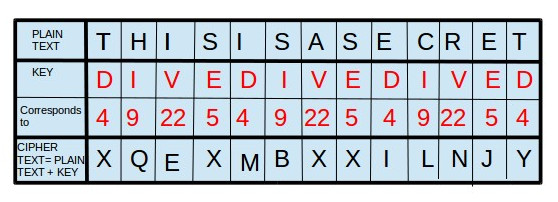
\includegraphics[width=0.9\textwidth]{vigenere.jpg}
\label{vigenere}
\caption{Working of Vigenere cipher}
\end{figure}

It can be seen as a combination of Caesar cipher and substitution cipher. Every alphabet of the plain text is shifted by a different number depending upon the letter of the key corresponding to that place. So, at some places, the same alphabet can be shifted by 5, rather at some places, it can be shifted by 22 and so on. Hence, the final result does not follow the frequency distribution of the English alphabets. 

\subsubsection{Cryptanalysis}

\textbf{Observe that} if the key length is known in the Vigenere cipher, then the cryptanalysis is straightforward. \\

\textbf{{\large How:-}}Assume that the length of the key is $l$, then we know that the alphabets at the locations $i$, $i+l$, $i+2l$, .... are shifted by the same number, since they all correspond to the same key letter. Example- In Figure \ref{vigenere}, the size of the key is 4. Hence, the alphabets at locations 1, 5, 9 and 13 are all shifted by the same number(4 corresponding to `D'). Similarly, alphabets at locations 2, 6 and 10 are shifted by same number(9 corresponding to `I') and so on. \\

So, if take the set of alphabets of cipher text at the locations $i$, $i+l$, $i+2l$, ...., they form an instance of the substitution cipher itself, where an alphabet is substituted by the same symbol or the same another alphabet since they are shifted by an equal number. If we look at the frequency distribution of this subset, it should follow the English frequency distribution. So, now we do the same thing as in the substitution cipher. Replace the maximum occurring alphabet in this subset of cipher text by `E', second maximum occurring by `T' and so on. \\

\[
 \boxed{\textbf{The\ question\ which\ still\ remains\ is\ how\ to\ find\ the\ key\ length?}}
 \]
 
\textbf{{\large Finding Key Length:-}} Let $S$ be a string of length $N$, where $N$ is a very large number, say $N = 10^6$. \\

$S = s_1\ s_2\ s_3\ ...\ s_{10^6-1}\ s_{10^6}$\\

Let $L$ be the number of letters in a language, for example, $L=26$ for English. \\

If we pick two letters from $S$, probability that they are same = \textbf{?}. \\

Number of ways in which two distinct letters can be picked from $S$ = $N \times (N-1)$ (considering ordered pair). Assume a letter $s_i$ occurs $p_i$ number of times in $S$. \\

Then probability that the picked letters $s_i$ and $s_j$ are same = $\sum_{i=1}^L \frac{(p_i) \times (p_i - 1)}{ N \times (N-1)}$ \\

We take the summation from $1$ to $L$ because the picked letter can be any letter from the set of letters of the language. \\

$\sum_{i=1}^L \frac{(p_i) \times (p_i - 1)}{ N \times (N-1)}$\\

= $ \frac{1}{ N \times (N-1)}\sum_{i=1}^L (p_i) \times (p_i - 1)$\\

= $ \frac{1}{ N \times (N-1)}\sum_{i=1}^L (f_i.N) \times (f_i.N\ - 1)$\\

= $ \frac{1}{N-1}\sum_{i=1}^L (f_i) \times (f_i\ - 1)$\\

= $\sum_{i=1}^L f_i \times f_i$		\hspace{5mm} since $N$ is a very large number\\

= $\sum_{i=1}^L {f_i}^2$\\

= $6.8 \times {10}^{-2}$, for English language\\

\textbf{How does this result help us?}: If the given text was to be random, instead of the massive text from English(or some other language), then all the $f_i$s would be the same. In that case\\	

$\sum_{i=1}^L {f_i}^2$\\

=$\sum_{i=1}^{26} {\frac{1}{26}}^2$\\

= $3.8 \times {10}^{-2}$  \\

This difference in both the cases helps us in finding the key length. Let us see how. \\

Given a cipher text, rotate the text by 1 letter and look at the number of collisions as shown in the Figure \ref{vigc}. Please note that the figure is used just to explain the rotation and counting concept. 

\begin{figure}[h]
\centering
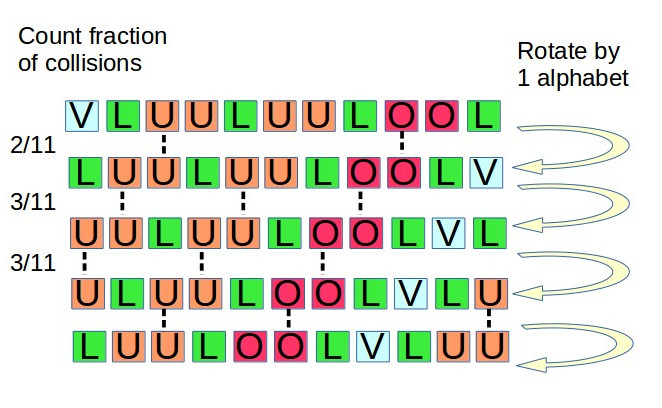
\includegraphics[width=0.9\textwidth]{vig_c.jpg}
\label{vigc}
\caption{Finding key length $l$ in vigenere cipher}
\end{figure}

As shown in the figure, we keep rotating the cipher text and look at the fraction of collisions. The mega result is : \\

\textbf{\textit{The fraction of collisions mostly is 3.8 \%, but as soon as the number of rotations becomes equal to the key length $l$, the fraction of collisions increases to 6.8\%.}} 
\end{document}